\documentclass[aspectratio=169,11pt]{beamer}

% ============================================================
% SISMID 2026 -- Day 2, 9:00 session
% Data beyond Google Trends (S. Yang + C. Djorno)
% Wikipedia pageviews + wastewater (CDC NWSS), scraped with the
% agent, continuing the Day 1 workflow.
% Compile: pdflatex data-beyond-google-trends.tex  (run twice)
% ============================================================

\IfFileExists{beamerthememetropolis.sty}{
  \usetheme{metropolis}
  \metroset{progressbar=frametitle, sectionpage=progressbar, numbering=fraction}
}{
  \usetheme{Boadilla}
  \usecolortheme{seahorse}
  \setbeamertemplate{navigation symbols}{}
}

\usepackage[utf8]{inputenc}
\usepackage[T1]{fontenc}
\usepackage{tikz}
\usetikzlibrary{arrows.meta, positioning, fit, backgrounds, calc}
\usepackage{xcolor}
\usepackage{listings}

\definecolor{AccentA}{HTML}{2A6F97}
\definecolor{AccentB}{HTML}{C1666B}
\definecolor{AccentC}{HTML}{3B8A5B}
\setbeamercolor{frametitle}{bg=AccentA}
\setbeamercolor{progress bar}{fg=AccentB}

\definecolor{skbg}{rgb}{0.96,0.96,0.94}
\lstdefinestyle{prompt}{
  basicstyle=\ttfamily\scriptsize,
  backgroundcolor=\color{skbg},
  showstringspaces=false, breaklines=true,
  frame=single, framesep=4pt, columns=fullflexible, numbers=none,
}
\lstset{style=prompt}

\tikzset{
  cbox/.style={draw=AccentA, very thick, rounded corners, align=center,
    minimum height=1.0cm, inner sep=6pt, font=\small, fill=AccentA!6},
  sbox/.style={draw=AccentA, thick, rounded corners, align=center,
    minimum height=0.85cm, inner sep=4pt, font=\scriptsize, fill=AccentA!6},
  rbox/.style={draw=AccentB, thick, rounded corners, align=center,
    minimum height=0.85cm, inner sep=4pt, font=\scriptsize, fill=AccentB!8},
  gbox/.style={draw=AccentC, thick, rounded corners, align=center,
    minimum height=0.85cm, inner sep=4pt, font=\scriptsize, fill=AccentC!8},
  flow/.style={-{Stealth[length=3mm]}, very thick, draw=AccentB},
  flowq/.style={-{Stealth[length=2.4mm]}, thick, draw=AccentA!70},
}

% flow cue: hand off from slides to the notebook
\newcommand{\tonb}[1]{\vspace{0.1em}\begin{flushright}\footnotesize\textcolor{AccentB}{$\blacktriangleright$~\textbf{#1}}\end{flushright}}

\title{Data Beyond Google Trends}
\subtitle{Wikipedia pageviews and wastewater, scraped with an agent}
\author{Shihao Yang \quad\textbullet\quad Candice Djorno}
\institute{SISMID 2026 \textbullet\ Day 2, 9:00}
\date{July 21, 2026}

\begin{document}

\begin{frame}
  \titlepage
\end{frame}

\begin{frame}{Why more than search}
  Yesterday you got fluent with \textbf{one} stream. Google Trends is powerful but has real
  blind spots: attention bias, English skew, sampling instability.
  \begin{block}{Today}
    Add two streams that fail \emph{differently}, so their errors do not line up:
    \textbf{Wikipedia pageviews} and \textbf{wastewater}. Same agent workflow, two new
    sources.
  \end{block}
  \vspace{0.3em}
  \begin{center}
  \resizebox{0.56\textwidth}{!}{%
  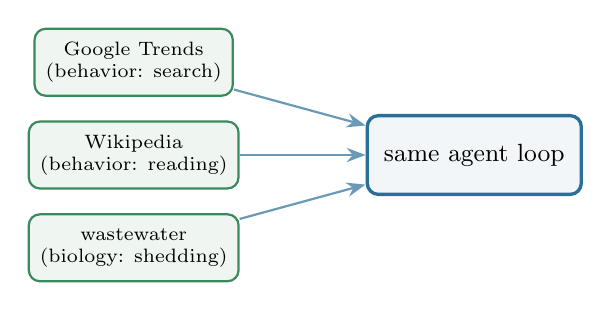
\begin{tikzpicture}[node distance=0.3cm and 1.2cm]
    \node[gbox] (g) {Google Trends\\(behavior: search)};
    \node[gbox, below=of g] (w) {Wikipedia\\(behavior: reading)};
    \node[gbox, below=of w] (s) {wastewater\\(biology: shedding)};
    \node[cbox, right=1.6cm of w] (a) {same agent loop};
    \draw[flowq] (g) -- (a); \draw[flowq] (w) -- (a); \draw[flowq] (s) -- (a);
  \end{tikzpicture}}
  \end{center}
\end{frame}

\begin{frame}{Roadmap}
  \tableofcontents
\end{frame}

% ===============================================================
\section{Google Trends revisited: the API}

\begin{frame}{First, let us fix yesterday}
  Before adding new streams, we repair the one you already know.
  \begin{itemize}
    \item Yesterday you scraped Google Trends with \texttt{pytrends} and met its two
          problems: \textbf{HTTP 429} rate limits, and values that \textbf{change between
          pulls}, because the public endpoint is \emph{sampled}.
    \item There is an official \textbf{Google Trends API}. It returns the \textbf{same
          normalized 0--100 index}, so nothing about your analysis changes.
  \end{itemize}
  \vspace{0.3em}
  \begin{center}
  \footnotesize
  \begin{tabular}{lll}
    \hline
     & \textbf{pytrends (scraping)} & \textbf{Trends API} \\
    \hline
    Access   & unofficial endpoint          & documented API, needs a key \\
    Failures & HTTP 429 roulette            & none in normal use \\
    Values   & \textbf{resampled each pull} & \textbf{identical every pull} \\
    Signal   & normalized 0--100            & \textbf{the same} 0--100 \\
    \hline
  \end{tabular}
  \end{center}
\end{frame}

\begin{frame}[fragile]{Unlock the class key}
  \begin{block}{In the terminal, before you start Jupyter}
  \begin{lstlisting}
source scripts/unlock-gt-api-key.sh
  \end{lstlisting}
  \end{block}
  Exports \texttt{GT\_API}. If Jupyter is open, \textbf{restart the kernel}.
  \begin{lstlisting}
GET https://www.googleapis.com/trends/v1beta/graph
    ?key=$GT_API
    &terms=dengue&terms=/m/0cycc      # terms OR topic ids
    &restrictions.geo=MX              # US, MX, US-GA ...
    &restrictions.startDate=2021-07   # YYYY-MM
    &restrictions.endDate=2026-07
  \end{lstlisting}
  \begin{itemize}
    \item \textbf{Quota: 1,000 requests/day for the whole room}, health topics only.
    \item Window length picks weekly vs monthly, exactly as on the website.
  \end{itemize}
\end{frame}

\begin{frame}{Term vs topic: why today needs topics}
  A \textbf{term} is the literal string. A \textbf{topic} is Google's Knowledge Graph entity
  (\texttt{/m/0cycc} = Influenza), folding together every spelling, synonym and
  \textbf{language}.
  \begin{center}
  \footnotesize
  \begin{tabular}{lcccc}
    \hline
    \textbf{Country} & \multicolumn{2}{c}{\textbf{term ``flu''}} & \multicolumn{2}{c}{\textbf{topic /m/0cycc}} \\
                     & max & mean & max & mean \\
    \hline
    United States & 88 & 22.1 & 100 & 24.9 \\
    France        & 3  & 0.9  & \textbf{100} & \textbf{16.3} \\
    Italy         & 4  & 1.6  & \textbf{100} & \textbf{17.7} \\
    Mexico        & 4  & 1.7  & \textbf{100} & \textbf{37.1} \\
    \hline
  \end{tabular}
  \end{center}
  \vspace{0.2em}
  \begin{center}
    \itshape An English term is nearly silent abroad. One topic id works in every language,
    which is what makes going multi-country today possible.
  \end{center}
  \tonb{Open \texttt{notebooks/00\_google\_trends\_api.ipynb} and pull your own topic.}
\end{frame}

\begin{frame}{What the API does not fix}
  The API makes the \emph{delivery} reliable. It does not change what search \emph{is}.
  \begin{itemize}
    \item Google Trends still measures \textbf{attention}, not infection: news coverage moves
          it too.
    \item Low-volume places still return a lot of \textbf{zeros}.
    \item The relationship to disease still \textbf{drifts} between seasons.
  \end{itemize}
  \vspace{0.3em}
  \begin{alertblock}{So we still need other streams}
    A reliable pipe does not make one signal sufficient. Next: streams that fail
    \emph{differently}, so their errors do not line up.
  \end{alertblock}
\end{frame}

% ===============================================================
\section{Wikipedia pageviews}

\begin{frame}{What Wikipedia pageviews are}
  A free, hourly log of how many times each article was viewed, exposed through one official
  \textbf{Wikimedia REST API} (no key).
  \begin{itemize}
    \item Views of ``Dengue fever'' or ``Influenza'' track public attention, much like
          search, but from a \textbf{different behavior}: reading, not querying.
    \item \textbf{Stable and reproducible}: pull the same series twice and the numbers match.
          A welcome contrast to Google Trends.
    \item Deep history (2015 onward), consistent methodology, well documented.
  \end{itemize}
  \vspace{0.3em}
  \begin{center}
    \itshape A dependable, well-behaved stream. Good to learn the multi-source workflow on.
  \end{center}
\end{frame}

\begin{frame}{Language is a feature}
  Wikipedia is per-language, so one concept gives you \textbf{several} signals at once.
  \begin{itemize}
    \item The \textbf{Spanish} article speaks for much of Latin America, \textbf{Portuguese}
          for Brazil, \textbf{English} for global attention.
    \item This is where Wikipedia beats Google Trends: strong \textbf{country-level} and
          \textbf{non-English} signal, exactly where search coverage is thin.
    \item A natural extra time series for the Dengue exercise: overlay the Spanish and
          Portuguese dengue articles on the case curve.
  \end{itemize}
  \vspace{0.3em}
  \begin{center}
    \itshape Pick the language that matches the population you are trying to see.
  \end{center}
\end{frame}

\begin{frame}[fragile]{Scrape it with the agent}
  Same five-step loop as yesterday. Only the fetch changes.
  \begin{block}{Prompt}
  \begin{lstlisting}
Using the Wikimedia REST pageviews API (no key, set a
descriptive User-Agent), pull daily views for the
"Dengue fever" article in English, Spanish, and
Portuguese since 2016. Use all-access and all-agents,
resolve redirects to the canonical title, align to
weekly, merge on date, plot the three, and report the
date range and any gaps.
  \end{lstlisting}
  \end{block}
  \begin{center}
    \itshape Then the habit: one plot, one sanity question, before it enters a model.
  \end{center}
\end{frame}

\begin{frame}{Wikipedia gotchas}
  \begin{itemize}
    \item \textbf{Article titles differ by language} and can be renamed; a wrong title
          silently returns nothing. Resolve to the canonical page and check the count is
          non-zero.
    \item \textbf{Access and agent filters matter}: \texttt{all-access} vs mobile/desktop,
          and \texttt{all-agents} vs \texttt{user} (exclude bots) change the series.
    \item \textbf{Attention spikes}: a news event or a linked front-page item can spike
          views with no change in disease, just like search.
    \item \textbf{Disambiguation}: ``Cold'' the illness vs the temperature. Prefer specific
          articles or topics.
  \end{itemize}
\end{frame}

% ===============================================================
\section{Wastewater surveillance (CDC)}

\begin{frame}{A fundamentally different kind of signal}
  Wikipedia and Google Trends measure \textbf{behavior}. Wastewater measures \textbf{biology}.
  \begin{itemize}
    \item Treatment plants are sampled for pathogen genetic material (viral RNA). It counts
          \textbf{shedding} by infected people, whether or not they search, test, or seek care.
    \item Because people shed early, it can \textbf{lead} clinical reporting, and it captures
          mild and asymptomatic cases that never reach a clinic.
    \item Publicly available from the CDC \textbf{National Wastewater Surveillance System
          (NWSS)}, by site and by jurisdiction.
  \end{itemize}
  \vspace{0.3em}
  \begin{center}
    \itshape The one stream here that does not depend on human attention at all.
  \end{center}
\end{frame}

\begin{frame}[fragile]{Scrape it with the agent}
  \begin{block}{Prompt}
  \begin{lstlisting}
From CDC's National Wastewater Surveillance System (NWSS)
open data on data.cdc.gov, pull the weekly wastewater
viral activity level for Georgia (state aggregate, and
list the reporting sites). Tidy to date + value, plot it,
and overlay a reference such as ILI or ED visits so I can
see whether it leads. Report site coverage and any gaps.
  \end{lstlisting}
  \end{block}
  \begin{center}
    \itshape The agent finds the dataset, handles the query, and returns a tidy series; you
    judge whether it actually leads.
  \end{center}
\end{frame}

\begin{frame}{Wastewater gotchas}
  \begin{itemize}
    \item \textbf{Coverage varies}: which plants report, and what fraction of the population
          they cover, changes over time and by state. Gaps are common.
    \item \textbf{Normalization}: raw concentration is adjusted for flow and for a fecal
          marker (PMMoV). Compare like with like; do not mix raw and normalized.
    \item \textbf{Single site is noisy}: a regional or state aggregate is far more stable
          than one plant.
    \item \textbf{Reporting lag and cadence}: it is fast, but not instant, and not every
          site reports every week.
  \end{itemize}
  \vspace{0.3em}
  \begin{alertblock}{Assess it honestly}
    The claim is early warning. Check the \textbf{lead time against ILI} yourself, as in
    Santillana's wastewater preprint, rather than assuming it.
  \end{alertblock}
\end{frame}

% ===============================================================
\section{Continuing the Day 1 workflow}

\begin{frame}{Same loop, same habits, now three streams}
  \begin{center}
  \resizebox{0.96\textwidth}{!}{%
  
\begin{tikzpicture}[node distance=0.9cm]
    \node[sbox] (f) {\textbf{fetch}\\the new API};
    \node[sbox, right=of f] (t) {\textbf{tidy}\\date + value};
    \node[sbox, right=of t] (p) {\textbf{plot}\\look first};
    \node[rbox, right=of p] (s) {\textbf{sanity-check}\\coverage, gaps};
    \node[gbox, right=of s] (v) {\textbf{save}\\tidy CSV};
    \draw[flow] (f) -- (t); \draw[flow] (t) -- (p); \draw[flow] (p) -- (s); \draw[flow] (s) -- (v);
  \end{tikzpicture}}
  \end{center}
  \vspace{0.4em}
  \begin{itemize}
    \item Nothing new to learn in the \emph{workflow}: describe the outcome, let the agent
          fetch, then verify. Only the source changed.
    \item Wikipedia and CDC are well-behaved (no datacenter block), so retries and the proxy
          rarely come up here. Google Trends was the hard one.
  \end{itemize}
\end{frame}

\begin{frame}{You now hold a small multi-stream bundle}
  For your disease and place, you can now assemble, side by side:
  \begin{itemize}
    \item Google Trends (search behavior), preprocessed,
    \item Wikipedia pageviews (reading behavior, multi-language),
    \item wastewater (biological shedding),
    \item all against a reference such as ILI or ED visits.
  \end{itemize}
  \vspace{0.3em}
  \begin{center}
    \itshape This bundle is the raw material for the capstone: independent signals whose
    errors do not line up.
  \end{center}
\end{frame}

\begin{frame}{Looking ahead}
  \begin{itemize}
    \item \textbf{Next (11:00):} more novel streams, human mobility (ground and air) and
          news alerts for emerging outbreaks.
    \item \textbf{This afternoon:} fold these signals into \textbf{ARGO}, alongside the
          disease's own history.
    \item \textbf{Day 3:} bring your own problem, and combine whichever streams fit it.
  \end{itemize}
  \vfill
  \begin{center}
    \itshape Two more streams down, the same loop each time. The library of signals is
    growing.
  \end{center}
\end{frame}

\begin{frame}[standout]
  Questions?\\[0.4em]
  \small Repo: \texttt{github.com/Shihao-Yang/sismid2026}
\end{frame}

\end{document}
